\documentclass[a4paper]{report}
\pagestyle{headings}
\usepackage{hyperref}
\usepackage{listings}
\usepackage{graphicx}
\usepackage{subfiles}
\usepackage{multirow}
\usepackage[table,xcdraw]{xcolor}
\lstset{numbers=right}
\lstset{breaklines}
\title{Lab Report for Software Engineering course \newline
 Lab 4: Starbubucks coffee online retailing system v3.0}
\author{Wang, Chen\qquad Liu, Jiaxing\qquad Huang, Jiani\qquad Tang, Xinyue \\
16307110064\qquad17302010049\qquad 17302010063\qquad 16307110476 \\
School of Software\\
Fudan University
}
\date{\today}
\bibliographystyle{plain}
\begin{document}
\maketitle

\tableofcontents
\chapter{Overview of this lab}
% Wang, Chen's part below
\section{The Objectives of the Project}
Through this experiment, we will experience the impact of demand changes on development work, experience the software project management functions provided by Huawei's development cloud platform DevCloud, and experience the rapid deployment of application services with SpringBoot.
\section{Specifications of the Lab}
The company now hopes that the development team will develop an \textbf{Online Beverage Sales System} based on the existing system. Based on the existing system, in addition to the existing \textbf{basic functions}, the \textbf{new requirements} are as follows:
\subsection{Add ingredients}
\begin{itemize}
\item
To meet the needs of our customers, we offer a wide range of ingredients including: milk, chocolate, cream and sugar.
\item
The price of adding a unit of milk and chocolate is \$1.2 for the price of the beverage; the price of the unit of cream and sugar is \$1 for the price of the beverage; and a portion of the beverage can be added with a plurality of ingredients.
\end{itemize}
\subsection{Adding drinks}
\begin{itemize}
\item
In order to meet the needs of customers, we offer a variety of drinks, and now we have added drinks, so that the system can provide coffee and tea sales, including cup type matching, ingredient addition, price calculation and so on.
\item
Coffee types now include: Espresso, Cappuccino; Tea varieties now include: Green Tea (GreenTea), Black Tea (RedTea).
\end{itemize}
\subsection{Price calculation}
Due to the adjustment of ingredients and drinks, the price calculation of drinks is adjusted accordingly.
\begin{itemize}
\item
The salesperson can choose the type of drink, the type of drink, or a variety of ingredients. The system will calculate the final price of the cup drink for the salesperson. The final price of the drink is calculated as follows: final price = drink price + drink cup type price + multiple ingredient price (unit: \$);
\item
The salesperson can select the number of cups under the premise of selecting a certain type of drink type. The system will calculate the final price of the multi-cup drink for the salesperson. The price is calculated as follows: multi-cup final price = single cup final price * cup number (unit :\$);
\item
Coffee and tea cups are currently divided into three types: large cup (3), medium cup (2), and small cup (1). Different cup types have different prices:
\end{itemize}
\begin{table}[htbp]
\center
\begin{tabular}{|l|l|l|}
\hline
\rowcolor[HTML]{575C61} 
{\color[HTML]{FFFFFF} \textbf{Large Cup}} & {\color[HTML]{FFFFFF} \textbf{Medium Cup}} & {\color[HTML]{FFFFFF}\textbf{Small Cup} } \\ \hline
Coffee Price +  \$6&Coffee Price +  \$4&Coffee Price +  \$2\\\hline
Tea Price +  \$5&Tea Price +  \$4&Tea Price +  \$2\\\hline
\end{tabular}
\end{table}
\subsection{Promotional programs}
In order to attract more customers at a more favorable price, the company now offers the following promotional strategies for different beverages selected by customers:
\subsubsection{The first category: combination offer}
\begin{itemize}
\item
Big cup Espresso, 20 cups off 2 cups (base price discount, 3 cups, 2 cups, 20 fold, 4 cups, 20\% off, and so on)
\item
RedTea/GreenTea (total) buy 3 get 1 free (buy 4 get 1 free, buy 5 get 1 free, buy 6 get 2 free, and so on)
\item 
Half price of Cappucino 2nd cup (half price of base price, half price of 1 cup in 2 cups, half price of 2 cups in 4 cups, and so on)
\end{itemize}
\subsubsection{The second category: full reduction offer}
\begin{itemize}
\item
All items are over \$100 minus 30\$ (over 200\$ minus 60\$ and so on)
\end{itemize}
\subsection{Basic price list}
The basic price list is shown as the table below.

\begin{table}[htbp]
\center
\begin{tabular}{|l|l|}
\hline
\rowcolor[HTML]{575C61} 
{\color[HTML]{FFFFFF} \textbf{Drink}} & {\color[HTML]{FFFFFF} \textbf{Basic Price}} \\ \hline
Espresso&\$20\\\hline
Cappuccino&\$22\\\hline
GreenTea&\$16\\\hline
RedTea&\$18\\\hline
\end{tabular}
\end{table}
\section{The division of work in the team}
\subsection{Division of work: Wang, Chen}
\subsubsection{(Git username: \emph{Wang, Chen}; Student ID: \emph{16307110064})}
He constructs the overall structure of the project, divides the entire workload into several parts so that each part can be finish the work separately. In addition, he draws the diagram of the entire project on the Huawei cloud platform that contains the parts like Epic, feature, story and tasks. Furthermore, he scratches the outline of how to implement the methods adopted in this project. At last, he summarized the general parts in the documentation and drafted some regulations for commit messages.

\subsection{Division: Huang, Jiani}
\subsubsection{(Git username: \emph{Currycurrycurry} Student ID: \emph{17302010063})}
She creates the concrete classes for the diverse drinks and ingredients.

\subsection{Division: Tang, Xinyue}
\subsubsection{(Git username: \emph{xinyuetang} Student ID: \emph{16307110476})}
She implements the methods related to order processing, discount processing and total price processing.

\subsection{Division: Liu, Jiaxing}
\subsubsection{(Git username: \emph{jiaxingliu} Student ID: \emph{17302010049})}
He tests the implementation in this project via the interface given by the teaching assistants.
\section{Division of work for documentation}
\subsection{Parts required in the documentation}
In the requirement documentation of the lab, we are required to accomplish the following parts in this documentation:
\begin{enumerate}
\item Explain the design ideas of work item planning in this experiment(PLAN);
\item Explain the design ideas of code implementation in this experiment(IMPLEMENT);
\item Explain the understanding of demand changes and project management (project planning, defect management, etc.) in this experiment(UNDERSTAND);
\item Explain the problems and solutions (if any) encountered in the implementation(PROBLEM).
\end{enumerate}
For the convenience of being noted, each requirement is labeled with a tag, which is used in the next part for mentioning.
\subsection{Principal for each part of the documentation}
\begin{table}[htbp]
\center
\begin{tabular}{|l|l|}
\hline
\textbf{Tag} & \textbf{Writer} \\ \hline
 PLAN&Wang, Chen\\ \hline
 IMPLEMENT&Huang, Jiani\&Tang, Xinyue\\ \hline
 UNDERSTAND&Wang, Chen\\ \hline
 PROBLEM&Liu, Jiaxing\\ \hline
\end{tabular}
\end{table}



% Wang, Chen's part below
\chapter{Improved skills on team collaboration}
\section{Consistent git commit message styles}
\subsection{Commit message requirements}
The following are the requirements for the commit message in our team, this version of specifications are revised according to the commit message style recommendation from website \emph{Commit message guidelines · GitHub}\footnote{Github contributors. (2019, March 22). Commit message guidelines. In \emph{GitHub, Inc}. Retrieved 14:53, April 28, 2019, from \url{https://gist.github.com/robertpainsi/b632364184e70900af4ab688decf6f53}}, \emph{How to Write a Git Commit Message}\footnote{Chris Beams. (2014, August 31). How to Write a Git Commit Message. In \emph{Chris Beams}. Retrieved 14:59, April 28, 2019, from \url{https://chris.beams.io/posts/git-commit/}}, \emph{How To Write a Good Commit Message}\footnote{The coala Developers. (2018). How To Write a Good Commit Message. In \emph{coala 0.12.0.dev20180614080551 documentation}. Retrieved 14:56, April 28, 2019, from\url{https://api.coala.io/en/latest/Developers/Writing_Good_Commits.html}} and the git commit message recommendation from one of the most authoritive open source project \textbf{GNOME} \emph{Guidelines for Commit Messages}\footnote{ZeeshanAli. (2019, March 18). Guidelines for Commit Messages. In \emph{GNOME Wiki!}. Retrieved 13:56, April 28, 2019, from\url{https://wiki.gnome.org/Git/CommitMessages}}.
\begin{enumerate}
\item
Only ASCII characters are allowed in the entire commit message
\item
All commit messages must start with one of the types identified in the following table, all words are lowercase
\item
It is best to have an associated work item, associated with the work item, followed by type, space \# number space followed by content, such as fix \#123 content
\item
The total number of characters recommended in the subject \emph{(note that it is the number of chars instead of the number of words)} is less than 50, and the maximum number is not more than 74 characters (including the previous type and item number, etc.)
\item
There is no need to add a period at the end of the head
\item 
After the type in the subject line, the first letter of the first word after the task number (if any) is capitalized and that indicates the beginning of a sentence
\item
Use the imperative tone in the subject sentence (although it is you who have actually done the work)
\item
The tense of the subject is the general present tense
\item
It is recommended that for commits involving complex modifications, body should be added in addition to the subject for further explanation. The method is as follows: break a new line and then write is the body, [do not follow the head without line break]
\item
For the body part of the commit message, there is no requirement other than writing Chinese, and it is relatively free. It is also recommended to write more than one line instead of one line in order to facilitate reading.
\end{enumerate}

\subsection{Types allowed in the subject of the commit message}

\newcommand{\tabincell}[2]{\begin{tabular}{@{}#1@{}}#2\end{tabular}}
\begin{table}[htbp]
\centering
\caption{\label{tab:test}Commit message types}
\begin{tabular}{|l|l|}
\hline
\textbf{Type} & \textbf{Description} \\ \hline
feat&A new feature\\ \hline
fix&A bug fix\\ \hline
wip&While working on a fix/feature\\ \hline
docs&Documentation only changes\\ \hline
style&\tabincell{c}{Changes that do not affect the meaning of the code \\(white-space, formatting, missing semi-colons, etc) }\\ \hline
refactor&A code change that neither fixes a bug or adds a feature\\ \hline
test&Adding missing tests \\ \hline
chore&\tabincell{c}{Changes to the build process or auxiliary tools \\and libraries such as documentation generation}\\ \hline
\end{tabular}
\end{table}
\section{API testing via Swagger}
\subsection{The Swagger API testing tool: Swagger Inspector}
Swagger is an open-source software framework backed by a large ecosystem of tools that helps developers design, build, document, and consume RESTful Web services. While most users identify Swagger by the Swagger UI tool, the Swagger toolset includes support for automated documentation, code generation, and test-case generation. 
\par
Sponsored by SmartBear Software, Swagger has been a strong supporter of open-source software, and has widespread adoption. 
\par
With Swagger Inspector, we can validate our APIs without any kind of setup or desktop downloads. We need to start testing immediately right in your browser. Tests are auto-saved so you can access them anywhere, anytime. Our Huawei Cloud account allows us to curate collections of tests and pin important endpoints to remember for later.
\section{Interface testing adopted in this project}
\subsection{API test case design in this project}
In this project, we designed the API test case shown in the following Figure \ref{1} configured on the Huawei Cloud platform. We sent a \emph{POST} request and then expected the price of the response.
\begin{figure}
\includegraphics[scale=0.4]{code.jpg}
 \caption{API test case}\label{1}
\end{figure}
\subsection{API test result of the interface}
The test result of the API testing is shown in the Figure \ref{2} below, which indicates that our project has passed the expected test cases.
\begin{figure}
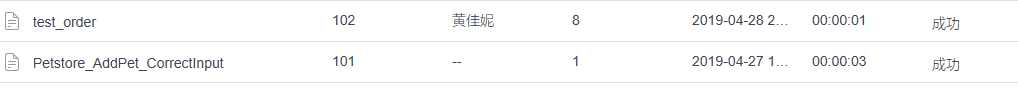
\includegraphics[scale=0.7]{result.png}
 \caption{API test result}\label{2}
\end{figure}
\chapter{Designed Ideas of work planning}
% Wang, Chen's part below
% 

There are two aspects to new requirements. One is the correctness of the original code, the other is the correctness of the new code. But this experiment is not entirely new development based on the original code, so there is no dedicated work item for the first point. For the new code part, considering the number of team members, we separated writing functional code from writing unit tests, avoiding the one-sided assumption of each member. Specifically, let one member set up the drinks storage class as a basis on which two other members work together to complete the new price calculation. This work plan is obtained.
\par

In this Lab, the work is divided according to the basic class realization, price calculation, discount calculation and test realization. Because essentially it is only a function of the pay method, so in this Lab, test work and development work are not integrated, but separated. This approach does not take advantage of the idea of driving test development, but it allows for increased communication between team members on DevCloud (more like a real development project), allowing us to maximize the use of DevCloud's project management and issue functionality on this project.

\par

This lab work item planning is mainly divided into two parts: commodity type storage and order price calculation. Commodity type storage: store some information about drinks in a reasonable way, mainly including drinks and ingredients, so the information about drinks and ingredients are packaged into categories for subsequent processing. Price calculation of orders: including the original price (excluding discount) and the final price calculation. At the same time, write test cases to test the price calculation may appear in a variety of circumstances.



% Wang, Chen's part above
\chapter{Design ideas of implementation}
\section{Entities implementation}
% Huang, Jiani's part below
The implementation of entity package can be divided into one package and one class: the package of drinkEntity and the class Ingredient.
\par At first, I apply this.getClass.getName() to simplify the constructor by avoiding inputting string every time. However, it is evident that the tedious information in className (the long package name) may cause other related problems. So in later modification, the constants created for drink-names in the class InfoConstant are used in the constructor method, which is also very simple and clear.
\subsection{drinkEntity}
\par At present we have four different kinds of drinks: Cappuccino,Espresso,GreenTea and RedTea. But considering the possibilities of adding other kinds of coffee and tea and the rationality of logic, the abstract classes of Coffee and Tea are applied to construct the whole inheritance relationship.That is, Both Coffee and Tea will inherit the OrderItem class, and all specific kinds of coffee and tea will inherit the abstract classes of Coffee and Tea.
\par We should pay attention to the constructor method of the different concrete classes. Since the initialization only need the different basic price of drinks, we only need to call the setPrice() method in constructor method. And all the generic method of these classes will be implemented in the parent class, the OrderItem class, such as cost() and size2price() methods.
Thanks to the inheritance tree, in the size2price() method, we can use the instanceof keyword to simplify the judge of cup-size.
\subsection{ingredientEntity}
At first I use four concrete ingredients inheriting the Ingredient class in dto package: chocolate, cream, milk and sugar. However, I realized that the concrete classes of ingredients actually are unnecessary. By using the API -- Hashmap and ArrayList, we can simplify the representation of different ingredients.
\subsection{OrderItem}
 Two methods are added for the class: size2price and cost in this class in order to make all its subclasses use this method.

% Huang, Jiani's part above
\section{Order services implementation}
% Tang, Xinyue's part below
\subsection{get total price of an order}
add a new function getTotalPrice() to the Order Class,which calculates the total price of an order and return it back. 
\par the logic of promotional functions.
\subsection{rule1:Twenty percent off for every two cups of large espresso}
count the number of large espresso in the order and save it in an int named by count,then the discount for espresso is (count/2)*0.2*20*2.
\subsection{rule2:buy 3 get 1 for free in tea sales}
count the number of GreenTea and RedTea and  save them in two ints named by countGreenTea and countRedTea.
Then the number of tea for free is (countGreenTea + countRedTea)/4.
To get largist discount, if the free cups of tea is less than the cups of RedTea(which is more expensive than GreenTea),
the discount of tea is countRedTea * 18. else the discount of tea is countRedTea * 18 + (freeNumber - countRedTea) * 16.
\subsection{rule3:The second cup of Cappuccino is half price}
count the number of Cappuccino in the order and save it in an int named by countCappuccino,then the discount for Cappuccino is (countCappuccino / 2)*22*0.5.
\subsection{compare the two kinds of promotion plan}
calculate the discount in the two kinds of promotion plan separately and choose the larger one.

% Tang, Xinyue's part above

\chapter{Understanding of demand changes}


This new addition to the demand for the new types of drinks and discount calculation. The impact of this change in project planning is to ensure that the original code is correct and that new functionality is added correctly. However, due to the particularity of this experiment, the operation of CSV was cancelled. Therefore, the original part of the code, such as the login and registration, was bound to change at the very beginning. Since there was no rigid requirement for this part in this requirement, the work in this part was cancelled in the project planning, and the new requirements were only developed. As for the defect management part, the strategy adopted is who finds who records, which is of great convenience for the later code inspection and can be implemented to specific personnel to solve the subsequent problems.

\par

Requirements change is a common problem in real development, sometimes it is the addition of new functions, and sometimes it is the total overthrow of a function again. Faced with such a situation, the design of the project will be particularly important, good design can easily solve these problems; On the other hand, if the design is not appropriate, resulting in code coupling is too strong, scalability is too bad, it will be difficult to cope with the change in requirements, resulting in the loss of time and manpower. Project management is essential when many people work together. A large project is decomposed into different blocks, which are respectively undertaken by different members. At the same time, establish work items and development tasks, and the development tasks are marked as pending, ongoing, testing and solving, etc., so as to effectively monitor the progress of the project and the work of each member, as well as effectively manage the defects of the project.


\par


The demand of lab has changed obviously compared with the last few times. For my part, due to the addition of ingredients and the increase in the types of drinks, as well as the change in the way of storing information related to drinks, the way of calculating the price is quite different from the previous one. Through this lab, I realized that the change of requirements is inevitable, so we must keep the good structure, style and modifiability of the code in the process of implementation, so that we can modify the code more conveniently when the requirements are changed later.

\par

Project planning is conducive to the logical thinking of the code, discussing the planning is to discuss the specific implementation of the code. Although the division of labor is different and the work is somewhat burdensome in the planning, at least this division of labor is logical and effective in my opinion, which has been proved to be the case. Defect management also made me realize that in the process of development, anyone's work is and others, which is closely linked with certain coupling, so there is a problem, need to deal with that part of the people and the corresponding communication, although we have WeChat can be directly said, but it will make records of trouble, so defects treatment is very good solve the problem, even after the problem again, can also go to previous administration reference before the situation to make corresponding analysis. This also facilitates the writing of the final document and the success of the test.




\chapter{Testing of the features}
\section{Testing methods adopted}
% Liu, Jiaxing's part below
Since the primary interface is the method \emph{pay} in class \emph{OrderServiceImpl}, the testing for the class is necessary. Given that the method is very complex and contains many factors, it's very nice to add a testing class for the class \emph{Order}.
\subsection {Testing for class Order}
\par To generate a legal order, I design a method \emph{getOrder}, which accepts some order items and return a order with an id generated with the date. And it's a helper method and it can reduce the repetition. Assuring that the total price computing is right is very important, so I design a method \emph{testGetTotalPriceOK} to test it, where I generate a order and check whether the return price is right. What's more, there may exist some unexpected exceptions. To be easy, I take three types of exception into account: the size of order items may be illegal, the order items may be null and the ingredients may be null. Well, there may be other unexpected exceptions. To make the  program much safer, I leave them in the other testing class. 
\par Many people may think the testing for the class is unnecessary, but it's not true. I think only the implementation of base functions is convincing, can we make a larger programn well.
\subsection {Testing for class OrderServiceImpl}
\par Compared with the former test class, it is much more important to generate a good testing class for class \emph{OrderServiceImpl}. Since the logic of promotional functions can be devided into two parts: the one of full reduction and the one of combination promotion. To assure each function is implemented well, I design some method to test them partly.
\par Testing for full reduction is very easy. I just generate a total price and pass it to the method \emph{fullReduction}. According the logic for full reduction, I can easily get the right discunt. So the next step is clear. I just need to check whether the return value is equal to the expected one. Here is the code:
  \begin{lstlisting}[language=java]
        assertEquals(orderService.fullReduction(160), 30.0, 0.01);
	\end{lstlisting}
\par Testing for combination promotion is much more complicated and I need take three situations into account. The three situations are twenty percent off for every two cups of large espresso, buy 3 get 1 for free in tea sales and the second cup of Cappuccino is half price. So there are three methods to test them and the key part is check whether the return discount is right.
\par Testing for the method pay is most important. I should design two orders which will partly choose two promotion strategies. According to the order, I can guess what the discount may be. So the next step is to check it. And the two testing methods are \emph{testPayWithFullReduction} and \emph{testPayWithCombination}.
\par Well, testings for some important fucntions are over, but there may be some unexpected exceptions. I take some exceptions into account: the order may be null, order.orderItems may be null, one of order.orderItems may be null, orderItem.ingredients may be null, one of orderItem.ingredients may be null and one of orderItem.ingredients may have illegal name or size. In fact, all the exceptions are generated by assertion statements. So to check the exception is to catch an instance of \emph{AssertionError} and check the message.

% Liu, Jiaxing's part above
\section{Testing results}
% Liu, Jiaxing's part below
Testing is to assure that our program is essentially safe and creditable, so it is very important. While testing, I find some problems and also some good ideas.
\subsection{Some problems}
\par The first problem I find is that if I want to check some key methods partly, I must modify their access rights. And I think it is very uncomfortable. On one hand, if not, the testing may be incomplete and may be very complex. On the other hand, if so, it will make the structure of the class worse. And it is very sad that now I still don't work out a good solution. And I choose the second choice to solve it. It's very nice that we finally find a good solution. I modify the testing methods and just test the oridinary interface without changing their access rights.
\par How about others? Well, I also find some bugs, such as the wrong implementation of the method \emph{fullReduction} which primarily return (totalPrice / 100) * 30 and be modify to return (int) ((totalPrice) / 100) * 30.0 later, the wrong using of some variables and stuff. But they do not matter, because it is very easy to correct. The most important thing is that it lacks some necessary exception checking in the implementation of these methods. And later we add them. 
% Liu, Jiaxing's part above
\subsection{Some good ideas}
\par In total, the methods to be tested are well implemented, especially the using of stream and labdma statements. And they can help make the program more efficent and more pithy. What's more, the design of them is very nice. I think tang has very good skills of designing methods and it is very helpful for my testing. The relationship of each methods is very fine and clear.
\chapter{Problems encountered and solutions}
\section{the Improper Use of getClass().getName() Method}
The first try to simplify the constructor method of entity classes proves to be infeasible.Since the whole project is composed of many organized packages, and this function will return a whole path string of the package name it belongs to, the class name we finally get will be long and confusing.
\par Thanks to the help of Jiaxing Liu, in the final version we decided to still use the string constants of drink names in constructor method. Every time we construct a new kind of drink class, we need to add the drink name in the infoConstant class.
\section{the Defect of Ingredient Class Design}
For each kind of ingredient, a unique class is applied at first, which bring about the problem of the concrete classes with only a few attributes (a bad design). 
\par Therefore, we use the key-value data structure -- map to represent each kind of ingredient, and arraylist for the total collection of ingredients added.

\begin{thebibliography}{A}


\bibitem{1}
Wikipedia contributors. (2019, March 22). JUnit. In \emph{Wikipedia, The Free Encyclopedia}. Retrieved 14:53, April 1, 2019, from \url{https://en.wikipedia.org/w/index.php?title=JUnit&oldid=888928403}

\end{thebibliography}
\end{document} 